\renewcommand{\theequation}{\theenumi}
\renewcommand{\thefigure}{\theenumi}
\renewcommand{\thetable}{\theenumi}
\begin{enumerate}[label=\thesection.\arabic*.,ref=\thesection.\theenumi]
\numberwithin{equation}{enumi}
\numberwithin{figure}{enumi}
\numberwithin{table}{enumi}

\item Let $U$ and $V$ be two independent zero mean Gaussian random variables of variances $\frac{1}{4}$ and $\frac{1}{9}$ respectively. The probability $\pr{3V \geq 2U}$ is \dots
\\
\solution
From the given information,
\begin{align}
    U &= \gauss{0}{\frac{1}{4}}
    V &= \gauss{0}{\frac{1}{9}}
\end{align}
%
Let $Y = 3V - 2U$.  Then, 
\begin{align}
   \mean{Y} &= 3\mean{V} - 2\mean{U} = 0
\\
\var{Y} &= 3^2\var{V} + 2^2\var{U} = 2
\end{align}
\begin{align}
    \therefore Y = \gauss{0}{2}
\end{align}
Thus, 
\begin{align}
    \pr{3V \geq 2U} &= \pr{3V-2U \geq 0}
    \\
    &= \pr{Y \geq 0} = \frac{1}{2}
\end{align}
$\because$ Y is symmetric about the origin.

%
\item $(X,Y)$ follows bivariate normal distribution $N_2$(0,0,1,1,$\rho$),  -1 $<$ $\rho$ $<$ 1. Then,
\begin{enumerate}
    \item $X+Y$ and $X-Y$ are uncorrelated only if $\rho$ = 0
    \item $X+Y$ and $X-Y$ are uncorrelated only if $\rho$ $<$ 0
    \item $X+Y$ and $X-Y$ are uncorrelated only if $\rho$ $>$ 0
    \item $X+Y$ and $X-Y$ are uncorrelated for all values of $\rho$
\end{enumerate}
\solution
Given that 
\begin{align}
 \vec{M} = \myvec{ X \\ Y}
 \sim  \gauss{\boldsymbol{\upmu}}{\boldsymbol{\Sigma}}
\end{align}
%
where 
%Here, Mean matrix of X and Y is:
\begin{align}
    \boldsymbol{\upmu} &= \myvec{0 \\ 0}
    \\
\boldsymbol{\Sigma} &= \myvec{
            1 & \rho\\
            \rho & 1 
        }
\end{align}
Also, 
\begin{align}
    X+Y &
    = \vec{A}^\top \vec{M}
    \\
    X-Y &
    =\vec{B}^\top \vec{M}
\end{align}
where
\begin{align}
 \vec{A} &= \myvec{1 \\ 1}, 
    \vec{B} &= \myvec{1 \\ -1}
\end{align}
% Defining Covariance in terms of expectation value:
% \begin{align}
%     Cov(X,Y)=& E[(X-\boldsymbol{\upmu}_x)(Y-\boldsymbol{\upmu}_y)] \\
%     =& E[(X-0)(Y-0)]\\
%     =& E(XY)
% \end{align}
Thus, 
\begin{align}
 Cov(X+Y,X-Y) =& \vec{A}^\top \boldsymbol{\Sigma} \vec{B} \\
    % =& \myvec{1 \\ 1}^\top
    % \myvec{
    %         1 & \rho\\
    %         \rho & 1 
    %     }
    %     \myvec{1 \\ -1}\\ 
    % =& \myvec{1+\rho \\ 1+\rho}^\top
    %     \myvec{1 \\ -1}\\
    % =& (1+\rho)-1(1+\rho) \\
    =&   0
\end{align}
% Note that 
% \begin{align}
% Var(X+Y) = Cov(X+Y , X+Y)\\ 
%  Var(X-Y)  = Cov(X-Y , X-Y)
% \end{align}
% Hence,
% \begin{align}
%     Var(X+Y) =&\vec{A^\top} \boldsymbol{\Sigma} \vec{A} \\
%         =& \myvec{1 \\ 1}^\top
%          \myvec{
%             1 & \rho\\
%             \rho & 1 
%         }
%         \myvec{1 \\ 1}\\
%     =& \myvec{1+\rho \\ 1+\rho}^\top
%         \myvec{1 \\ 1}\\
%     =& 1+\rho+1+\rho \\
%     =& 2+2\rho \neq 0
% \end{align}
% \begin{align}
%     Var(X-Y) =& \vec{B^\top} \boldsymbol{\Sigma} \vec{B} \\
%         =& \myvec{1 \\ -1}^\top
%     \myvec{
%             1 & \rho\\
%             \rho & 1 
%         }
%          \myvec{1 \\ -1}\\
%     =& \myvec{1-\rho \\ \rho-1}^\top
%         \myvec{1 \\ -1}\\
%     =& 1-\rho-\rho+1 \\
%     =& 2-2\rho \neq 0
% \end{align}
% So correlation coefficient is:
% \begin{align}
%     \rho(X+Y,X-Y) = \frac{Cov(X+Y,X-Y)}{\sqrt{var(X+Y) \times var(X-Y)}}
%     = 0
% \end{align}
$\therefore$ X+Y and X-Y are uncorrelated irrespective of value of $\rho$ where $\rho \in \brak{-1,1}$.
%$\therefore$ The correct answer is \textbf{option 4}.
%
\item Let $U$ and $V$ be two independent zero mean Gaussian random variables of variances $\frac{1}{4}$ and $\frac{1}{9}$ respectively. The probability $\pr{3V \geq 2U}$ is \dots
\\
\solution
From the given information,
\begin{align}
    U &= \gauss{0}{\frac{1}{4}}
    V &= \gauss{0}{\frac{1}{9}}
\end{align}
%
Let $Y = 3V - 2U$.  Then, 
\begin{align}
   \mean{Y} &= 3\mean{V} - 2\mean{U} = 0
\\
\var{Y} &= 3^2\var{V} + 2^2\var{U} = 2
\end{align}
\begin{align}
    \therefore Y = \gauss{0}{2}
\end{align}
Thus, 
\begin{align}
    \pr{3V \geq 2U} &= \pr{3V-2U \geq 0}
    \\
    &= \pr{Y \geq 0} = \frac{1}{2}
\end{align}
$\because$ Y is symmetric about the origin.

%
\item Let $X_1,X_2,X_3,X_4,X_5$ be a random sample of size 5 from a population having standard normal distribution. If 
\begin{align}
    \label{gauss/3/mean}
    \overline{X}&=\frac{1}{5}\sum_{i=1}^5 X_i
    \\
    T &=\sum_{i=1}^5\brak{X_i-\overline{X}}^2
    \label{gauss/3/var}
\end{align}
%
then $\mean{T^2\overline{X}^2}$ is equal to 
\begin{enumerate}
    \item 3
    \item 3.6
    \item 4.8
    \item 5.2
\end{enumerate} 
\solution
\begin{lemma}
    \label{gauss/3/xy}
Let 
\begin{align}
    \vec{x}=\myvec{X_1\\
             X_2\\
             X_3\\
             X_4\\
             X_5}
, 
             \vec{y}=\myvec{Y_1\\
             Y_2\\
             Y_3\\
             Y_4\\
             Y_5}, 
             \sim \gauss{\vec{0}}{\vec{I}}
             \\
% \end{align}
% and 
% \begin{align}
    \vec{u}&=\myvec{1\\ 1\\ 1\\ 1\\ 1}, 
    \vec{v}=\myvec{1\\ 1\\ 1\\ 1\\ 0}.
\end{align} 
%
Then 
\begin{align}
    \overline{X}&=\frac{1}{5}\vec{u}^{\top}\vec{x}
    \\
    T &= \norm{\vec{v}^{\top}\vec{y}}^2
    \label{gauss/3/T}
\end{align}
where
\begin{align}
\vec{y} &= \vec{P}\vec{x}, 
\\
\vec{M} &= \vec{I}- \frac{1}{5}\vec{1}
\\
&= \vec{P}^{\top}\vec{D}\vec{P}, 
\\
    \vec{D} &=\myvec{1&0&0&0&0\\
                   0&1&0&0&0\\
                   0&0&1&0&0\\
                   0&0&0&1&0\\
                   0&0&0&0&0}
\end{align}
% \begin{align}
% %     \vec{M}&=\myvec{\frac{4}{5}&-1/5&-1/5&-1/5&-1/5\\
% %                    -1/5&\frac{4}{5}&-1/5&-1/5&-1/5\\
% %                    -1/5&-1/5&\frac{4}{5}&-1/5&-1/5\\
% %                    -1/5&-1/5&-1/5&\frac{4}{5}&-1/5\\
% %                    -1/5&-1/5&-1/5&-1/5&\frac{4}{5}}
% \vec{M} = \vec{I}- \frac{1}{5}\vec{1}
%  \end{align}
  and $\vec{1}$ is the all ones matrix.
\end{lemma}
%
\begin{proof}
From  \eqref{gauss/3/mean} and  \eqref{gauss/3/var}, it is easy to verify that 
\begin{align}
       T&=\vec{x}^{\top}\vec{M}\vec{x},
    \vec{M}^2=\vec{M}
    \\
    \implies T&=\vec{x}^{\top}\vec{P}\vec{D}\vec{P}^{\top}\vec{x}\\
    &=\vec{y}^{\top}\vec{D}\vec{y}
\end{align}
yielding     \eqref{gauss/3/T}.  We have used spectral decomposition above.
%
\end{proof}
\begin{lemma}    
    \label{gauss/3/orth}
    $\vec{y}=\vec{P}\vec{x} \sim \gauss{\vec{0}}{\vec{I}}$ if $\vec{P}^{\top}\vec{P} = \vec{I}$.
\end{lemma}
\begin{proof}
    The  moment generating function 
    \begin{align}
        M_{\vec{x}}\brak{\vec{t}}=exp\brak{\vec{t}^{\top}\vec{\mu}+\frac{1}{2}\vec{t}^{\top}\vec{V}\vec{t}}
    \end{align}
    $\because \vec{\mu}=\vec{0}$ and $\vec{V}=\vec{I}$,
    \begin{align}
         M_{\vec{x}}\brak{\vec{t}}=\exp\brak{\frac{1}{2}\vec{t}^{\top}\vec{t}}\label{gauss/3/2.11}
    \end{align}
    Therefore the joint moment generating function of $\vec{y}$ is
    \begin{align}
        M_{\vec{y}}\brak{\vec{t}}&=M_{\vec{x}}\brak{\vec{P}\vec{t}}\\
        &=exp\brak{\frac{1}{2}\vec{t}^{\top}\vec{P}^{\top}\vec{P}\vec{t}}
        \\
        &= M_{\vec{x}}\brak{\vec{t}}
    \end{align}
%    on comparing with $\eqref{gauss/3/2.11}$ we can say $\vec{y}$ has multivariate normal distribution. 
    \end{proof}
    \begin{corollary}
        \label{gauss/3/xbar}
        $\overline{X} \sim \gauss{0}{\frac{1}{5}}$
    \end{corollary}

    \begin{definition}
        \begin{enumerate}
        \item {\em Random Variable:} A random variable X is a real-valued function defined on the "sample space" $\Omega$ (the set of outcomes being studied via probability).
        \item {\em Borel Set:} A random variable X is studied by means of the probabilities that its value lies within various intervals of real numbers (or, more generally, sets constructed in simple ways out of intervals: these are the Borel measurable sets of real numbers).         
        \item {sigma-algebra: }  Corresponding to any Borel measurable set I is the event $X^*(I)$ consisting of all outcomes $\omega$ for which $X(\omega)$ lies in I.
        The sigma-algebra generated by X is determined by the collection of all such events.
        \item {\em Independent random variables: } The naive definition says two random variables X and Y are independent "when their probabilities multiply." That is, when I is one Borel measurable set and J is another, then 
        \begin{multline}
            \pr{X(\omega)\in I , Y(\omega)\in J}\\=\pr{X(\omega)\in I}\pr{Y(\omega)\in J}.
        \end{multline}
        But in the language of events (and sigma algebras) that's the same as
        \begin{multline}
            \pr{\omega \in X^*(I) , \omega \in Y^*(J)}\\=\pr{\omega \in X^*(I)}\pr{\omega \in Y^*J)}.
        \end{multline}
        \item {\em Function of a random variable: }
        \begin{align}
            (f\circ X)(\omega)&=f(X(\omega))
            \\
            (f\circ X)^*(I)&=X^*(f^*(I))
            \label{eq:gauss/3/omega}
        \end{align}
        \end{enumerate}
    
    \end{definition}
    
\begin{lemma}
    Functions of independent random variables are themselves independent.
    \end{lemma}
    \begin{proof}
     Consider now two functions $f,g:\mathbb{R}\rightarrow \mathbb{R}$ and suppose that $f\circ X$ and $g\circ Y$ are random variables. 
    In other words, every event generated by $f\circ X$ (which is on the left) in         \eqref{eq:gauss/3/omega} is automatically an event generated by X (as exhibited by the form of the right hand side). Therefore         \eqref{eq:gauss/3/omega} automatically holds for $f\circ X$ and $g\circ Y$.
    This covers the case of vector-valued random variables as well.
    \end{proof}
    \begin{corollary}
        Let $\vec{y}$ and $\vec{z}$ be two independent normal random vectors. Then $\vec{y}$ and $\vec{\norm{z}}$ are also independent.
    \end{corollary}

    \begin{lemma}
        \label{gauss/3/t2.3}    
        $\vec{A}\vec{x}, \vec{B}\vec{x}$ are  independent  if and only if $\vec{A}\vec{B}^{\top}=0$
        \end{lemma}
        \begin{proof}
        The given vectors are independent $\iff$ 
        \begin{multline}
            \mean{\brak{\vec{A}\vec{x}-\mean{\vec{A}\vec{x}}}\brak{\vec{B}\vec{x}-\mean{\vec{B}\vec{x}}}^{\top}} = 0\\
             \implies \vec{A}\mean{\brak{\vec{x}-\mean{\vec{x}}}\brak{\vec{x}-\mean{\vec{x}}}^{\top}}\vec{B}^{\top} = 0\\
             \implies \vec{A}\var{\vec{x}}\vec{B}^{\top} = 0\\
             \text{or, } \vec{A}\vec{B}^{\top} = 0, \quad \because \var{\vec{x}} = \vec{I}
        \end{multline}        
        \end{proof}
\begin{theorem}    
    $\vec{u}^{\top}\vec{x}$ and $\vec{v}^{\top}\vec{y}$ are independent.
\end{theorem}
\begin{proof}
    From Lemma     \ref{gauss/3/xy}, 
    \begin{align}
        \vec{y} = \vec{P}\vec{x}. 
    \end{align}        
The given statement can be proved  using Lemma         \ref{gauss/3/t2.3} and noting that      
    \begin{align}
        \vec{u}^{\top}\vec{P}^{\top} \vec{v}=0, 
    \end{align}            
\end{proof}
\begin{corollary}    
    $\overline{X} and T$ are independent.
\end{corollary}
    % \begin{conjecture}
    %     \label{l2.1/gauss/3/}
    %     For any vectors $\vec{u}, \vec{v}$, 
    %     \begin{align}
    %        \brak{\vec{u}^{\top}\vec{x}}\brak{\vec{x}^{\top}\vec{v}}=\vec{u}^{\top}\brak{\vec{x}\vec{x}^{\top}}\vec{v}
    %     \end{align}
    % \end{conjecture}
\begin{definition}
    \label{gauss/3/chisq}
    {\em chi-square distribution: } $\norm{\vec{x}}^2$ is said to be chi-square distributed.  If the length of $\vec{x}$ is $k$,
 The mean and variance are given by
 \begin{align}
   \mean{Y}&=k\\
   \var{Y}&=2k
 \end{align}
\end{definition}
From       Corollary  \ref{gauss/3/xbar} and      Definition \ref{gauss/3/chisq},
\begin{align}
    \mean{\overline{X}^2} &= \frac{1}{5}, 
    \\
    \mean{T^2} &=  \var{T}+\brak{\mean{T}}^2\\
    &=24
    \\
    \implies  \mean{T^2\overline{X}^2}=4.8
\end{align}
%
\item Suppose $(X_1,X_2)$ follows a bivariate  normal distribution with
\begin{align}
    &E(X_1)=E(X_2)=0\\
    &V(X_1)=V(X_2)=2\\
    &Cov(X_1,X_2)=-1
\end{align}
If $\Phi(x)$=$\frac{1}{ \sqrt{2\pi}}\int_{-\infty}^{x}e^{-\frac{{y}^2}{2}}\, dy$, then $\pr{X_1-X_2>6}$ = ?
\begin{enumerate}
    \item $\Phi(-1)$
    \item $\Phi(-3)$
    \item $\Phi(\sqrt{6})$
    \item $\Phi(-\sqrt{6})$
\end{enumerate}
\solution
\begin{definition}
    $\vec{x}\sim\mathcal{N}(\mu_{\vec{x}},\Sigma_{\vec{x}})$ is a bivariate random vector given by
    \begin{align}
        \vec{x}&=\myvec{X_1\\
                       X_2}\\
        \vec{\mu_{\vec{x}}}&=\myvec{\mu_1\\
                                    \mu_2}\\
        \vec{\Sigma_{\vec{x}}}&=\myvec{\sigma_1^2&\rho\sigma_1\sigma_2\\
                                        \rho\sigma_1\sigma_2&\sigma_2^2}
    \end{align}
    where $\vec{\Sigma_{\vec{x}}}$ is covariance matrix of $\vec{x}$ and $\rho$ is correlation of $X_1$ and $X_2$ which is given by
    \begin{align}
        \rho=\frac{\cov{X_1}{,X_2}}{\sigma_1\sigma_2}
    \end{align}
\end{definition}
\begin{lemma}
    \label{gauss/4/stats}
    Let $\vec{x}$ be a $K\times1$ multivariate normal random vector with mean $\vec{\mu}_x$ and covariance matrix $\vec{\Sigma_{\vec{x}}}$. Let $\vec{a}$ be an $L\times1$ real vector and $\vec{B}$ an $L\times K$ full rank real matrix with $K>L$ .Then the $L\times1$ random vector $\vec{y}$ defined by
    \begin{align}
        \vec{y}=\vec{a}+\vec{B}\vec{x}
    \end{align}
    has a multivariate normal distribution with mean
    \begin{align}
        \vec{\mu_\vec{y}}=\vec{a}+\vec{B}\vec{\mu_x}
    \end{align}
    and covariance matrix
    \begin{align}
        \vec{\Sigma_y}=\vec{B}\vec{\Sigma_x}\vec{B}^{\top}
    \end{align}
\end{lemma}
\begin{proof}
   The joint moment generating function of $\vec{x}$ is
   \begin{align}
       M_{\vec{x}}(\vec{t})&=\mathbb{E}[\exp{\brak{\vec{t}^{\top}\vec{x}}}]\\
       \implies M_{\vec{x}}(\vec{t})&=\exp{\brak{\vec{t}^{\top}\vec{\mu_x}+\frac{1}{2}\vec{t}^{\top}\vec{\Sigma_x}\vec{t}}}
   \end{align}
   $\therefore$, the joint moment generating function of $\vec{y}$ is
   \begin{align}
       M_{\vec{y}}(\vec{t})&=\mathbb{E}[\exp{\brak{\vec{t}^{\top}\vec{y}}}]\\
                           &=\mathbb{E}[\exp{\brak{\vec{t}^{\top}\brak{\vec{a}+\vec{B}\vec{x}}}}]\\ &=\exp{\brak{\vec{t}^{\top}\vec{a}}}\mathbb{E}[\brak{\vec{t}^{\top}{\vec{B}\vec{x}}}]\\ &=\exp{\brak{\vec{t}^{\top}\vec{a}}}\mathbb{E}[\brak{\vec{B}^{\top}\vec{t}}^{\top}\vec{x}]\\
                           &=\exp{\brak{\vec{t}^{\top}\vec{a}}}M_{\vec{x}}(\vec{B}^{\top}\vec{t})
        \end{align}
        which can be expressed as
        \begin{multline}
            M_{\vec{y}}(\vec{t})     \\                      =\exp{\brak{\vec{t}^{\top}\vec{a}}}\exp{\brak{(\vec{B}^{\top}\vec{t})^{\top}\vec{\mu_x}+\frac{1}{2}(\vec{B}^{\top}\vec{t})^{\top}\vec{\Sigma_x}\vec{B}^{\top}\vec{t}}}\\
                           =\exp\brak{\vec{t}^{\top}(\vec{a}+\vec{B}\vec{\mu_x})+\frac{1}{2}\vec{t}\vec{B}\vec{\Sigma_x}\vec{B}^{\top}\vec{t}^{\top}}
        \end{multline}
   
   which is the moment generating function of a multivariate normal distribution with mean $\vec{a}+\vec{B}\vec{\mu}$ and covariance matrix $\vec{B}\vec{\Sigma_x}\vec{B}^{\top}$.\\
   
   $\therefore$ $\vec{\mu_\vec{y}}=\vec{a}+\vec{B}\vec{\mu_x}$ and $\vec{\Sigma_y}=\vec{B}\vec{\Sigma_x}\vec{B}^{\top}$
\end{proof}
\begin{theorem}\label{1.1}
   If $(X_1,X_2)$ follows a bivariate distribution then 
   \begin{align}
    \pr{X_1-X_2>\alpha}=\Phi\brak{\frac{-(\alpha+\vec{u}^{\top}\vec{\mu_{\vec{x}})}}{\sqrt{\vec{u}^{\top}\vec{\Sigma_{\vec{x}}}\vec{u}}}}
   \end{align}
\end{theorem}
\begin{proof}
   Let $\vec{u}=\myvec{-1\\
                       1}$ and $\vec{x}=\myvec{X_1\\
                                           X_2}$.  Then 
   \begin{align}
       Y = X_2-X_1=\vec{u}^{\top}\vec{x}
   \end{align}
%    Now consider a random variable Y defined as follows
%    \begin{align}
%        Y&=X_2-X_1\\
%        \implies y&=\vec{u}^{\top}\vec{x}
%    \end{align}
%   then $Y$ has normal distribution with mean
with 
   \begin{align}
       \mu_{y}&=\vec{u}^{\top}\vec{\mu_{\vec{x}}} \\
%    \end{align}
%    and variance is given by
%    \begin{align}
       \sigma^2_{y}&=\vec{u}^{\top}\vec{\Sigma_{\vec{x}}}\brak{\vec{u}^{\top}}^{\top}\\
       \implies \sigma^2_{y}&=\vec{u}^{\top}\vec{\Sigma_{\vec{x}}}\vec{u}
       \\
       \text{or, } Y&\sim\mathcal{N}(\vec{u}^{\top}\vec{\mu_{\vec{x}}},\vec{u}^{\top}\vec{\Sigma_{\vec{x}}}\vec{u})
   \end{align}
   from Lemma     \ref{gauss/4/stats}.  Also, 
   \begin{align}
    Z  = \frac{Y-\mu_y}{\sigma_y} \sim \mathcal{N}(0,1) 
   \end{align}
   Thus, 
   
%    The Standard Normal, often written Z, is a Normal with $\mu=0$ and $\sigma^2=1$. Thus, $Z \sim \mathcal{N}(\mu=0,\sigma^2=1)$\\
%    Now $\pr{X_1-X_2>\alpha}$ can be written as $\pr{Y<-\alpha}$
   \begin{align}
       \pr{Y<-\alpha}&=\pr{\frac{Y-\mu_y}{\sigma_y}<\frac{-\alpha-\mu_y}{\sigma_y}}\\
       &=\pr{Z<\frac{-(\alpha+\vec{u}^{\top}\vec{\mu_{\vec{x}})}}{\sqrt{\vec{u}^{\top}\vec{\Sigma_{\vec{x}}}\vec{u}}}}
    \end{align}
    \begin{align}
       \implies  \pr{X_1-X_2>\alpha}=\Phi\brak{\frac{-(\alpha+\vec{u}^{\top}\vec{\mu_{\vec{x}})}}{\sqrt{\vec{u}^{\top}\vec{\Sigma_{\vec{x}}}\vec{u}}}}
       \label{gauss/4/temp}
   \end{align}
\end{proof}
   From the given information,
   \begin{align}
    \mu_1=\mu_2&=0\\
    \sigma^2_1=\sigma^2_2&=2\\
    Cov(X_1,X_2)&=-1\\
    \rho=\frac{Cov(X_1,X_2)}{\sigma_1\sigma_2}&=\frac{-1}{2}\\
    \vec{\mu_{\vec{x}}}=\myvec{\mu_1\\
                                    \mu_2}&=\myvec{0\\
                                                  0}\\
     \vec{\Sigma_{\vec{x}}}=\myvec{\sigma_1^2&\rho\sigma_1\sigma_2\\
                                        \rho\sigma_1\sigma_2&\sigma_2^2}&=\myvec{2&-1\\
                                                                                -1&2}
\end{align}
which, upon substituting in        \eqref{gauss/4/temp} yields 
\begin{align}
    \implies \pr{X_1-X_2>6}&=\Phi\brak{\frac{-6}{\sqrt{6}}}\\
    &=\Phi(-\sqrt{6})
\end{align}
%    \begin{lemma}
%        \begin{align}
%            \mu_{y}&=\vec{u}^{\top}\vec{\mu_{\vec{x}}}\\
%            \implies \mu_{\vec{y}}&=\myvec{-1\,\,1}\myvec{\mu_1\\
%                                                      \mu_2}\\
%            \implies \mu_{\vec{y}}&=\myvec{\mu_2-\mu_1}
%        \end{align}
%    \end{lemma}
%    \begin{lemma}
%        \begin{align}
%        \sigma^2_{y}&=\vec{u}^{\top}\vec{\Sigma_{\vec{x}}}\vec{u}\\
%        \implies \sigma^2_{y}&=\myvec{-1\,\,1}\myvec{\sigma^2_1&\rho\sigma_1\sigma_2\\
%                                                         \rho\sigma_1\sigma_2&\sigma^2_2}\myvec{-1\\
%                                                                                                1}\\
%        \implies \sigma^2_{y}&=\myvec{\sigma^2_1+\sigma^2_2-2\rho\sigma_1\sigma_2}
%        \end{align}
%    \end{lemma}
%    \begin{align}
%        \therefore \pr{X_1-X_2>\alpha}&=\Phi\brak{\frac{(\mu_1-\mu_2)-\alpha}{\sqrt{\sigma^2_1+\sigma^2_2-2\rho\sigma_1\sigma_2}}}
%    \end{align}
 %\end{proof}
% Given $(X_1,X_2)$ follow a bivariate normal distribution with
% \begin{align}
%    \mu_1=\mu_2&=0\\
%    \sigma^2_1=\sigma^2_2&=2\\
%    Cov(X_1,X_2)&=-1\\
%    \rho=\frac{Cov(X_1,X_2)}{\sigma_1\sigma_2}&=\frac{-1}{2}
% \end{align}
% for $\pr{X_1-X_2>6}$ we can use the above theorem as follows
% \begin{align}
%    \pr{X_1-X_2>\alpha}&=\Phi\brak{\frac{(\mu_1-\mu_2)-\alpha}{\sqrt{\sigma^2_1+\sigma^2_2-2\rho\sigma_1\sigma_2}}}\\
%    \implies \pr{X_1-X_2>6}&=\Phi\brak{\frac{(0-0)-6}{\sqrt{2+2-2\brak{\frac{-1}{2}}2}}}\\
%    \implies \pr{X_1-X_2>6}&=\Phi\brak{\frac{-6}{\sqrt{6}}}\\
%    \therefore \pr{X_1-X_2>6}&=\Phi(-\sqrt{6})
% \end{align}


\item Suppose
$\begin{pmatrix}
X\\
Y
\end{pmatrix}$ is a random vector such that the marginal distribution of $X$ and the marginal distribution of $Y$ are the same and each is normally distributed with mean 0 and variance 1. Then, which of the following conditions imply independence of $X$ and $Y?$
\begin{enumerate}
\item Cov$\brak{X,Y}=0$
\item $aX+bY$ is normally distributed with mean 0 and variance $a^2+b^2$ for all real $a$ and $b$
\item $\pr{X\le 0, Y\le 0}=\frac{1}{4}$
\item $E\sbrak{e^{itX+isY}}=E\sbrak{e^{itX}}E\sbrak{e^{isY}}$ for all real $s$ and $t$
\end{enumerate}
%
\solution


An important property of dirac delta function that will be used at multiple ocassions in this solution is
\begin{align}
\displaystyle\int\limits_{-\infty}^{\infty} f(x)\delta(x-a)dx=f(a) \label{dec/2015/109/eq:dirac}
\end{align}
Given $X\sim N\brak{0,1}, Y\sim N(0,1)$
\begin{enumerate}
\item
\begin{align}
Cov(X,Y)=0\\
E\sbrak{XY}-E\sbrak{X}E\sbrak{Y}=0\\
E\sbrak{XY}=0\\
\displaystyle \int\limits_{-\infty}^{\infty} \int\limits_{-\infty}^{\infty}xyf_{XY}(x,y) dxdy=0
\end{align}
This doesn't imply independence. Counter example given below\\
Lets consider a case where $X$ and $Y$ are dependent based on the following relation, $Y$ being independent of $K$
\begin{align}
X=KY \label{dec/2015/109/eq:case}
\end{align}
PMF for $K$ is given as
\begin{align}
p_K(k)=
\begin{cases}
\frac{1}{2} &k=1\\
\frac{1}{2} & k=-1\\
0 & \text{otherwise}
\end{cases}
\end{align}
A simulation is given below, Y is gaussian, then X also follows gaussian
\begin{figure}[!ht]
\centering
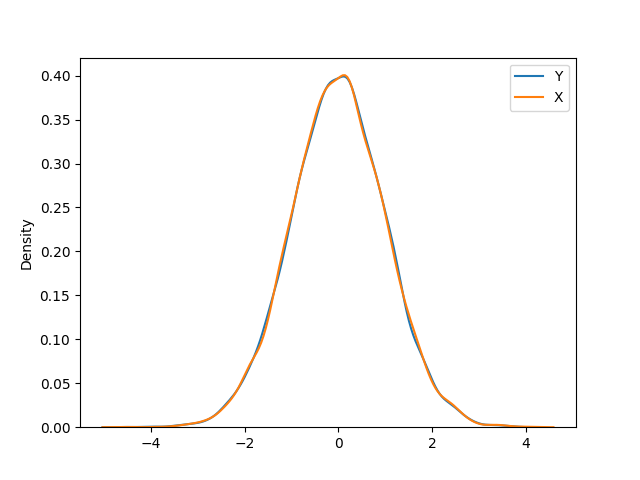
\includegraphics[width=\columnwidth]{solutions/2015/dec/109/figure/fig.png}
\caption{X and Y, if Y is normal}
\label{fig:dec/2015/109/plot}
\end{figure}
Theoretically it can be proved in the following manner,
Since $K$ and $Y$ are independent
\begin{align}
f_X(x)&=\pr{K=1}f_Y(x)+\pr{K=-1}f_Y(-x)\\
&=\frac{1}{2}\brak{f_Y(x)+f_Y(-x)}\\
&=f_Y(x)
\end{align}
Therefore, $X$ follows identical but not independent distribution as $Y$, An alternative proof is given below as a proof for marginal probability\\
Now consider that $X$ is normally distributed, we will establish $Y$ is also normally distributed.
The joint probability distribution is therefore
\begin{align}
f_{XY}(x,y)&=f_{X|Y}(x|y)f_X(x)\nonumber \\
&=f_X(x)\frac{1}{2}(\delta(x+y)+\delta(x-y))\label{dec/2015/109/eq:counter}
\end{align}
The marginal probability distribution function for $X$ is given as
\begin{align}
\int\limits_{-\infty}^{\infty}f_X(x)\frac{1}{2}(\delta(x+y)+\delta(x-y)) dy
\end{align}
Using \eqref{dec/2015/109/eq:dirac}, we get
\begin{align}
\int\limits_{-\infty}^{\infty}f_X(x)\frac{1}{2}(\delta(x+y)+\delta(x-y))dy=f_X(x)
\end{align}
We know that $X\sim N(0,1)$, $f_X(x)$ represents gaussian probability distribution function.\\
Futher, using symmetry of \eqref{dec/2015/109/eq:case}, we can establish that marginal distribution of $Y$ is gaussian. Here is a proof anyways
\begin{align}
f_Y(y)=\int\limits_{-\infty}^{\infty}f_X(x)\frac{1}{2}(\delta(x+y)+\delta(x-y)) dx
\end{align}
Using \eqref{dec/2015/109/eq:dirac}, we get
\begin{align}
f_Y(y)=\frac{1}{2}\brak{f_X(y)+f_X(-y)}=f_X(y)
\end{align}
Since $Y$ has identical probability distribution function, $Y\sim N(0,1)$\\
The covariance is given as
\begin{align}
&Cov(X,Y)=E[XY]-E[X]E[Y]=E[XY]\\
&E[XY]=\int\limits_{-\infty}^{\infty}\int\limits_{-\infty}^{\infty}xyf_{XY}(x,y) dy dx
\end{align}
\begin{align}
=\int\limits_{-\infty}^{\infty}\int\limits_{-\infty}^{\infty}xyf_X(x)\frac{1}{2}(\delta(x+y)+\delta(x-y)) dy dx\\
=\int\limits_{-\infty}^{\infty} xf_X(x)\int\limits_{-\infty}^{\infty}y\frac{1}{2}(\delta(x+y)+\delta(x-y)) dy dx
\end{align}
Using \eqref{dec/2015/109/eq:dirac}
\begin{align}
E[XY]=\int\limits_{-\infty}^{\infty}xf_X(x)\frac{1}{2}(x-x)dx=0
\end{align}
\item
Defining the following matrices/vectors
\begin{table}[h!]
\centering
\begin{tabular}{ |c|c|} 
\hline
\textbf{vector/matrix} & \textbf{expression} \\
\hline&\\[-1em]
$\boldsymbol{Z}$& $\begin{pmatrix} X &Y\end{pmatrix}^\top$\\[2pt]
\hline&\\[-1em]
$\boldsymbol{C}$&$\begin{pmatrix} a &b\end{pmatrix}^\top$  \\[2pt]
\hline&\\[-1em]
$\boldsymbol{\mu}$&$\begin{pmatrix} 0 &0\end{pmatrix}^\top$  \\[2pt]
\hline&\\[-1em]
$\boldsymbol{\Sigma}$&$\begin{pmatrix}1&\rho\\\rho&1\end{pmatrix}$ \\
\hline
\end{tabular}
\caption{vectors/matrices and their expressions}
\label{dec/2015/109/table1}
\end{table}
Given
\begin{align}
\boldsymbol{C^\top Z}\sim N\brak{0,a^2+b^2}
\end{align}
Since this is true for all $a$ and $b$, it is equivalent to $X$ and $Y$ being jointly gaussian
\begin{align}
\boldsymbol{Z}\sim N(\boldsymbol{\mu},\boldsymbol{\Sigma})
\end{align}
For correlated random variables $X$ and $Y$ in bivariate normal distribution, we have
\begin{align}
\sigma_{Z}^2=\displaystyle\sum_{i,j}\Sigma_{ij}\\
a^2+b^2=a^2+b^2+2\rho ab\\
\therefore \rho=0\label{dec/2015/109/eq:rho}
\end{align}
The joint distribution is given as
\begin{align}
f_{\boldsymbol{Z}}(x,y)=\frac{\text{exp}\brak{-\frac{1}{2}\brak{\boldsymbol{z-\mu}}^\top\boldsymbol{\Sigma}^{-1}\brak{\boldsymbol{z-\mu}}}}{\sqrt{(2\pi)^2\abs{\boldsymbol{\Sigma}}}}\\
f_{\boldsymbol{Z}}(x,y)=\frac{\text{exp}\brak{-\frac{1}{2}{\begin{pmatrix} x &y\end{pmatrix}} I_2{\begin{pmatrix} x &y\end{pmatrix}}^\top}}{\sqrt{(2\pi)^2}}
\end{align}
Where $I_2$ is the identity matrix of order 2
\begin{align}
f_{\boldsymbol{Z}}(x,y)=\frac{\text{exp}\brak{-\frac{1}{2}{\begin{pmatrix} x &y\end{pmatrix}} {\begin{pmatrix} x &y\end{pmatrix}}^\top}}{\sqrt{(2\pi)^2}}\\
f_{\boldsymbol{Z}}(x,y)=\frac{\text{exp}\brak{-\frac{1}{2}\brak{x^2+y^2}}}{\sqrt{(2\pi)^2}}=f_X(x)f_Y(y)
\end{align}
$\therefore$ \textbf{Option(2) is correct}, A simulation for bivariate gaussian is given below
\begin{figure}[!ht]
\centering
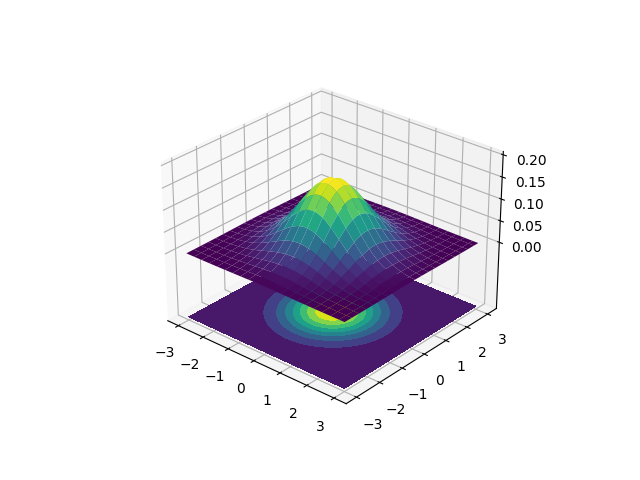
\includegraphics[width=\columnwidth]{solutions/2015/dec/109/figure/plot.png}
\caption{bivariate gaussian while 0 mean vector and identity covariance matrix}
\label{dec/2015/109/plot}
\end{figure}
\item
\begin{align}
\pr{X\le 0, Y\le0}=\frac{1}{4}
\end{align}
This doesn't imply independence, it can be true even for dependent $X$ and $Y$, the counter example is \eqref{dec/2015/109/eq:counter}, the joint probability function is symmetric across all 4 quadrants
\begin{align}
\therefore \pr{X\le 0, Y\le0}=\frac{1}{4}
\end{align}
Alternatively, here is proof 
\begin{align}
\pr{X\le 0}=F_X(0)=\frac{1}{2} \label{dec/2015/109/eq:pr1}
\end{align}
Using \eqref{dec/2015/109/eq:case}
\begin{align}
\pr{Y\le 0|X\le 0}=\frac{1}{2} \label{dec/2015/109/eq:pr2}
\end{align}
Using \eqref{dec/2015/109/eq:pr1} and \eqref{dec/2015/109/eq:pr2}
\begin{align}
\pr{X\le 0, Y\le0}=\frac{1}{4}
\end{align}
\item
\begin{align}
E\sbrak{e^{itX+isY}}=E\sbrak{e^{itX}}E\sbrak{e^{isY}}\\
E\sbrak{e^{itX+isY}}=\varphi_X(t)\varphi_Y(s) \label{dec/2015/109/eq:inde}
\end{align}
The inverse is given as
\begin{align}
f_{XY}(x,y)=\frac{1}{4\pi^2}\displaystyle \int\limits_{-\infty}^{\infty} \int\limits_{-\infty}^{\infty} e^{-itX-isY}E\sbrak{e^{itX+isY}}ds dt
\end{align}
Using \eqref{dec/2015/109/eq:inde}
\begin{align}
f_{XY}(x,y)&=\frac{1}{4\pi^2}\displaystyle \int\limits_{-\infty}^{\infty} \int\limits_{-\infty}^{\infty} e^{-itX-isY}\varphi_X(t)\varphi_Y(s) ds dt\\
&f_{XY}(x,y)=f_X(x)f_Y(y)
\end{align}
$\therefore$ \textbf{Option(4) is correct}
\end{enumerate}




\end{enumerate}